\documentclass{minimal}
\usepackage[paperwidth=6.3in,paperheight=2.18in,margin=0.05in]{geometry}
%\usepackage[paperwidth=6.1in,paperheight=3.53in,margin=0.05in]{geometry}

\usepackage[utf8]{inputenc}
\usepackage{amsmath}
\usepackage{amsfonts}
\usepackage{amssymb}

\usepackage{tikz}
\usetikzlibrary{matrix,chains,positioning,decorations.pathreplacing,arrows}
%%%%%%%%%%%%%%%%%%%%%%%% tikz packaque
%\usepackage{tikz}
\usetikzlibrary{shapes.geometric, arrows}
\tikzstyle{startstop} = [rectangle, rounded corners, minimum width=3cm, minimum height=1cm,text centered, draw=black, fill=red!30]
\tikzstyle{process} = [rectangle, minimum width=1cm, minimum height=1cm, text centered, draw=black, fill=orange!30]
\tikzstyle{process_2} = [rectangle, minimum width=2cm, minimum height=1cm, text centered, text width=4cm, draw=black, fill=orange!30]
\tikzstyle{process_3} = [rectangle, minimum width=2cm, minimum height=1cm, text centered, text width=2cm, draw=black, fill=orange!30]
\tikzstyle{process_4} = [rectangle, minimum width=1cm, minimum height=1cm, text centered, text width=1.2cm, draw=black, fill=orange!30]
\tikzstyle{arrow} = [thick,->,>=stealth]
%%%%%%%%%%%%%%%%%%%
\newcommand{\mbbU}{\mathbb{U}}
\newcommand{\mbbV}{\mathbb{V}}
\newcommand{\mbbR}{\mathbb{R}}
\DeclareMathOperator*{\argmin}{argmin}
%%%%%%%%%%%%%%%%%%%

\begin{document}


\begin{center}
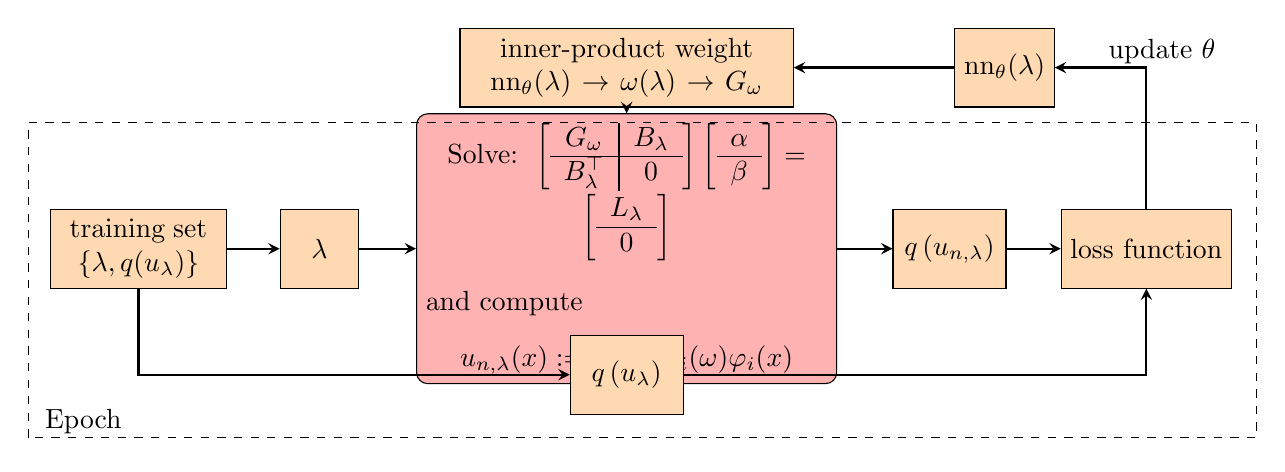
\begin{tikzpicture}[node distance=1.3cm]
%\draw[step=1cm,gray,very thin] (-7,-3) grid (11,3);
%
\node (mix_form) [startstop] {\begin{minipage}[t]{5.1cm} %\vspace*{-0.2cm}
\begin{center}
$ 
\text{Solve: }\left[\begin{array}{c|c}
G_{\omega} & B_{\lambda} \\
\hline
B_{\lambda}^{\top} & 0 
\end{array}
\right]
\left[\begin{array}{c}
\alpha \\ \hline \beta 
\end{array}
\right]
=
\left[\begin{array}{c}
L_{\lambda} \\ \hline 0
\end{array}
\right]
$ 
\end{center}
and compute
\begin{center}
$u_{n,\lambda}(x):= \sum_{i=1}^{n} \beta_i(\omega)\varphi_i(x)$
\end{center}
%\vspace*{-0.2cm}
\end{minipage}};
%
\node (omega) [process_2, above of=mix_form, yshift=1.0cm] {inner-product weight \\ $\mathrm{nn}_{\theta}(\lambda) \rightarrow \omega(\lambda) \rightarrow G_{\omega}$};
\node (lambda) [process, left of=mix_form, xshift=-2.6cm] {$\lambda$};
\node (train_set) [process_3, left of=lambda, xshift=-1.0cm] {$\mathrm{training\; set}$ $\left\{\lambda,q(u_{\lambda})\right\}$ %$\text{   or   }$ $\left\{\lambda,v_{m,q,\lambda}\right\}$ 
};
\node (qoi) [process_4, right of=mix_form, xshift=2.8cm] {$q\left(u_{n,\lambda}\right)$ %$\text{  or  }$ $r_{m,\lambda}$
};
\node (theta) [process, right of=omega, xshift=3.5cm] {$\mathrm{nn}_{\theta}(\lambda)$};
\node (loss) [process, right of=qoi, xshift=1.2cm] {loss function};
\node (qoi_ts) [process_4, below of=mix_form, yshift=-0.3cm] {$q\left(u_{\lambda}\right)$ %$\text{  or  }$ $v_{m,q,\lambda}$
};

%
\draw [arrow] (theta) -- (omega);
\draw [arrow] (omega) -- (mix_form);
\draw [arrow] (lambda) -- (mix_form);
\draw [arrow] (mix_form) -- (qoi);
\draw [arrow] (qoi) -- (loss);
\draw [arrow] (train_set)-- (lambda);
\draw [arrow] (train_set) |- (qoi_ts);
\draw [arrow] (qoi_ts) -| (loss);
\draw [arrow] (loss) |- (theta);
%\draw [dashed] (-7,-1.5) rectangle (10.5,1.5);
\draw [dashed] (-7.6,-2.4) rectangle (8.0,1.6);
%
\draw (-6.9,-2.2) node {Epoch};
\draw (6.8,2.5) node {update $\theta$};
%\draw (-5.6,0.8) node {Training set};
%
\end{tikzpicture}
\end{center}

\end{document}